To test our module that computes power and delay, we run some simulation changing $V_{DD}$ and fan-out according the three different technology families in the same year. In figure \ref{fig:fan-out_plot} is plotted the behavior of delay in function of fan-out.
\begin{figure}[htbp]
\begin{center}
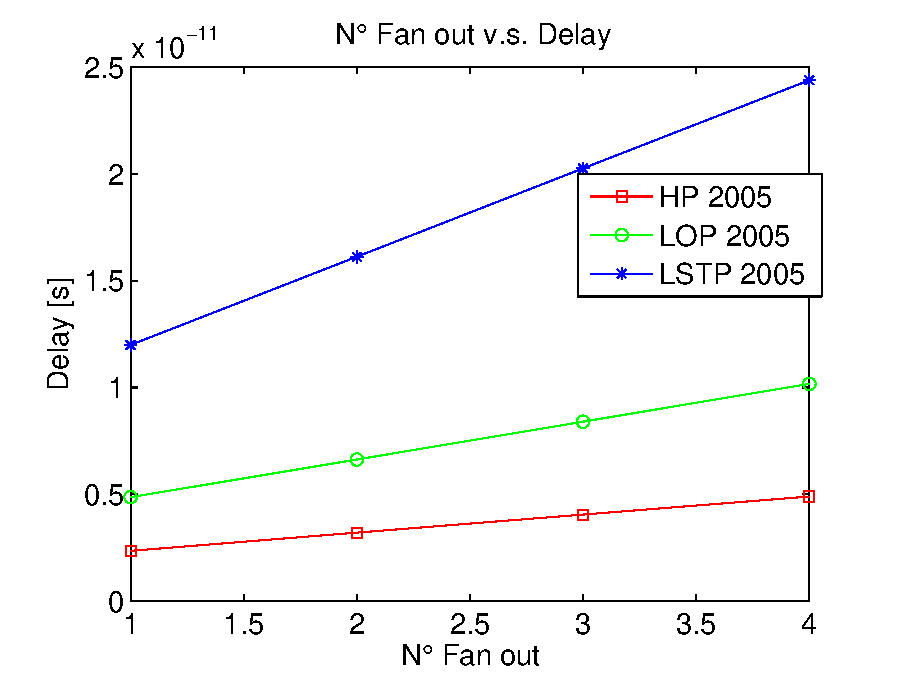
\includegraphics[width=0.8\textwidth]{img/plot_fanout_delay.eps}
\caption{Fan-out vs delay}
\label{fig:fan-out_plot}
\end{center}
\end{figure}
As we expected, increasing the fan-out, the delay increases too and find out also that HP technology has lower delay respect to LOP and LSTP, moreover its slope is less than other two. \\In figure \ref{fig:vdd_plot} is shown the delay variations for different $V_{DD}$ values according the three technology families.
\begin{figure}[htbp]
\begin{center}
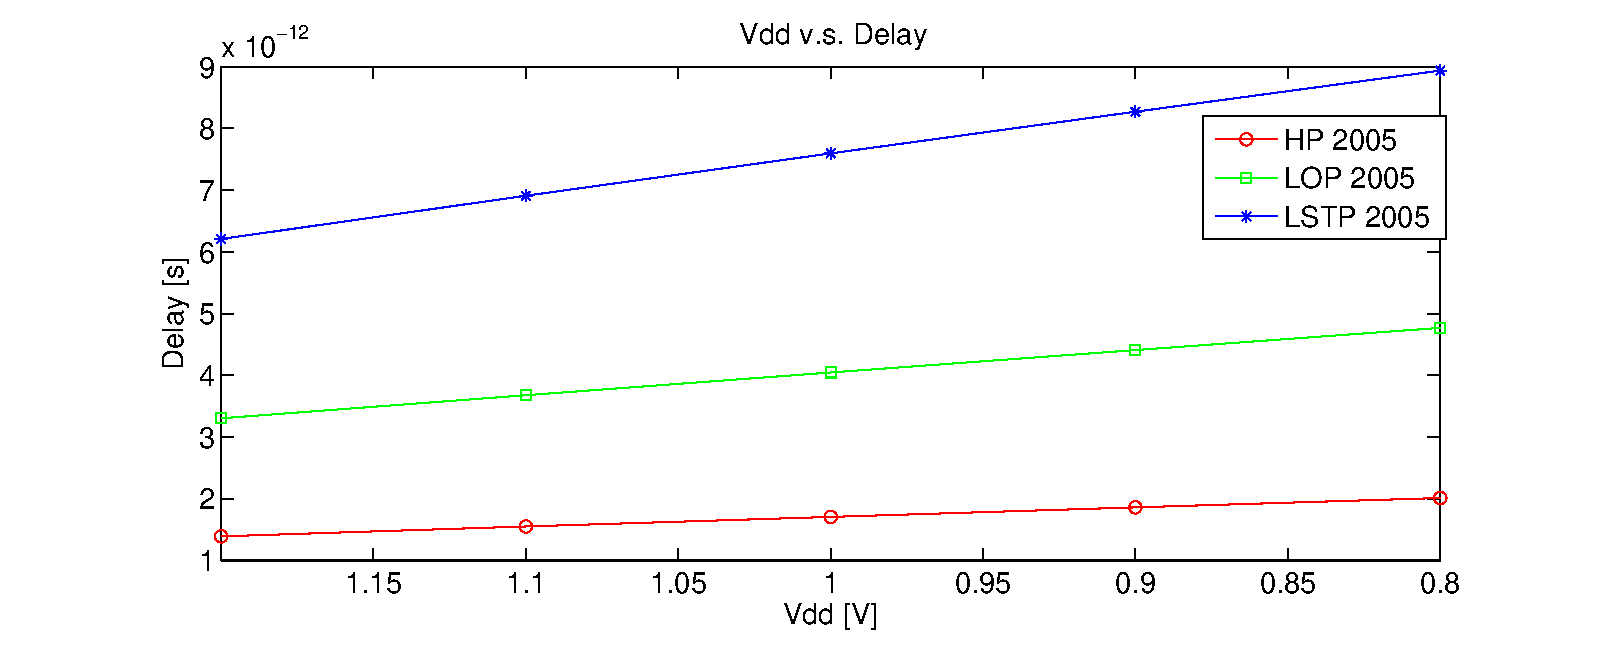
\includegraphics[width=0.8\textwidth]{img/plot_vdd_delay.eps}
\caption{$V_{DD}$ vs delay}
\label{fig:vdd_plot}
\end{center}
\end{figure}
As we expected, delay increases as $V_{dd}$ decreases. As before, the slope of HP is lower than the other two but less compared to fan-out plot. \\About power, in table \ref{tab:power} are reported static and dynamic power for the three families at 2005.
\vspace{2cm}
\\
\textbf{NOTE:} Variable Cox received in input at our module should be in $pF/\mu m^2$, but we have verified that must be multiplied by 10 to have a correct Cox.
\begin{table}[htdp]
\begin{center}
\begin{tabular}{|c|c|c|c|}
\hline
 & HP [W] & LOP [W] & LSTP [W]\\
\hline
P static & $3.7411\cdotp 10^{-4}$ & $2.3884\cdotp 10^{-6}$ & $1.6137\cdotp 10^{-8}$\\
\hline
P dynamic & $2.518\cdotp 10^{-6}$ & $1.3937\cdotp 10^{-6}$ & $2.4310\cdotp 10^{-6}$\\
\hline
\end{tabular}
\end{center}
\caption{Static and dynamic power for 2005 technological node}
\label{tab:power}
\end{table}